
\documentclass[10pt]{ietbook}
\usepackage{listings}
\begin{document}

%For RH Book title
\rhbooktitle{Advances in Weather Radar}
%\setminted[python]{breaklines, framesep=2mm, fontsize=\footnotesize, numbersep=5pt}

\markboth{}

\cauthor{Mircea Grecu\thanks{GESTAR-II, Morgan State University and NASA GSFC} and\\
William S. Olson\thanks{GESTAR-II,UMBC and NASA GSFC} }

\chapter{Satellite Combined Radar-Radiometer algorithms}

Some abstract here.
\section{Introduction}

The benefit of incorporating radiometer observations into methodologies that estimate precipitation from
space-borne radar observations was first realized by \cite{weinman90}. Specifically, due to size and weight limitations on antennae, space-borne radars 
operate at frequencies that make observations subject to attenuation. While
attenuation correction methodologies exist, e.g. \cite{hitschfeld1954}, variability in the size distribution of
precipitation particles within the radar observing volume makes the attenuation correction process highly uncertain.
At the same time, it had been recognized \cite{Meneghini1983} that independent information regarding the Path-Integrated-Attenuation (PIA) 
may be used to reduce uncertainties in the attenuation correction process. PIA information
independent of the radar measurements used in the attenuation correction process may be derived from the analysis
of the electromagnetic power backscattered by the Earth's surface \cite{Meneghini1983} and, as noted by Weinman et al. \cite{weinman90}, 
low-frequency radiometer observations when available.  The objective of the surface analysis is to estimate the power backscattered by Earth's surface in the 
absence of the rain.  In the presence of rain, the ratio between the actual backscattered power and the estimated clear-sky backscattered power provides an estimate
of the total attenuation from the radar to the Earth's surface \cite{Meneghini1983} that can be used in attenuation correction and precipitation estimation process. 
The problem with the PIA estimation using this approach, usually referred to as the Surface Reference Technique (SRT), is that the estimation of the no-precipitation 
backscattered power may be highly uncertain in some situations.  As recognized by Weinman et al. \cite{weinman90} and even earlier investigators, e.g. \cite{Fujita1985},
radiometer observations over water surfaces at frequencies not associated with significant scattering (e.g. 10- and 19-GHz) contain information strongly related to the PIA.  
This is because the emissivity of water surface is low and rain drops in the radiometer observing volume result in warmer brightness temperatures.  The departure from the
brightness temperature value expected in clear skies may be used to estimate the equivalent PIA at the radar operating frequency \cite{weinman90}.  The initial study of
Weinman et al. \cite{weinman90} provided a relationship between coincident radiometer observations at X-band and the associated PIA at X-band (9.6-GHz). Subsequent work 
Smith et al. \cite{smith1997} was carried out to determine a relationship between the PIA at Ku-band (13.8 GHz) and coincident radiometer observations 10.7-GHz. 
This relationship was developed for use in the Tropical Rainfall Measuring Mission (TRMM) \cite{kummerow1998} combined radar-radiometer algorithm \cite{haddad1997}.

However, although the relationships between low frequency brightness temperatures and the radar PIA at X- and Ku-band are well-defined and unambiguous, the use of satellite
radiometer observations in satellite radar profiling algorithms is challenging. This because the typical footprints of low-frequency radiometer observations are significantly
larger than the typical footprints of space-borne radars, which makes the radiometer observations difficult to translate into radar PIA. To overcome this difficulty various
approaches akin to the downscaling of the radiometer observations to the radar footprint resolution have been developed \cite{haddad1997,grecu2004,masunaga2005,munchak2011}.
A common feature of these approaches was that the radar-footprint PIA was not directly estimated from the radiometer observations. Instead, 
optimization procedures were used to maximize the agreement between radiometer observations predicted from the radar observations and actual radiometer observations.  While
the impact of the radiometer observations on the final radar estimates is difficult to quantify, a clear benefit of combined radar-radiometer precipitation retrievals
are consistent with both the radar and radiometer observations.  Consequently, they may be used to derive large databases of precipitation and associated radiometer observations
necessary in the development of “Bayesian” precipitation estimation algorithms from satellite
radiometer-only observations \cite{grecu2006,kummerow2011,hou2014}. 

\section{Fundamental Models}

\subsection{Precipitation particles and their electromagnetic properties}

To numerically characterize integral properties of precipitation (such as the precipitation rate) within a radar observing volume, a good understanding of the 
distributions of properties such as the size and mass of precipitation particles is necessary.
Paramount to this is the concept of Particle Size Distribution (PSD).  Mathematically, the PSD is a function $N(D)$ that describes the density of precipitation particles of
a given size within an elementary atmospheric volume.  More precisely, $N(D)dD$ is defined as the concentration of precipitation particles with sizes between $D$ and $D+dD$
in a specified volume of air.  Given expressions that relate the size of a precipitation particle to its mass and electromagnetic backscattering
properties, the PSD function may be used to derive relationships between the Liquid Water Content (LWC) and radar reflectivity.  In a seminal
study, Marshall and Palmer  \cite{marshall_palmer_1948} showed that rain Drop Size Distributions (DSDs) follow an exponential distribution,
i.e. $N(D)=N_0\exp(-\lambda D)$.  Although subsequent studies showed that DSDs are generally better described by gamma functions,
$N(D)=N_0 D^{\mu}\exp(-\lambda D)$, (see Ulbrich 
\cite{ulbrich1983} for a review), the exponential DSD formulation of \cite{marshall_palmer_1948} represented a milestone in meteorology because
it set the stage for analytical investigations of the relationships between precipitation properties and radar observations.  While initially
focused preponderantly on rain, as measurement techniques improved, PSD studies started addressing ice particles in the early seventies 
(e.g. \cite{ssrivastava1970,heymsfield_a1977}). It was found that, similarly to raindrops, ice PSDs may be accurately described by gamma functions.

Equally important to the description of PSDs is the quantification of the amount of radar power backscattered by precipitation particles. 
To simplify the analysis, the radar measurements of returned power are converted into a related variable called the equivalent 
radar reflectivity factor, defined as:

\begin{equation} \label{eq:Z}
Z=\frac {\lambda ^4} {\pi ^5 |K_w|^2} \int_0^{\infty} N(D) \sigma _b(D) dD
\end{equation}
where $\lambda$ is radar frequency, $|K_w|$ is the dielectric factor of water, and $\sigma _b(D)$ is the 
backscattering cross-section of a precipitation particle of diameter $D$.  The backscattering cross-section is the equivalent area that
would isotropically return an amount of power equal to that actually returned by the precipitation particle \cite{battan1973}.  
The equivalent reflectivity factor is defined to equal $\int_0^{\infty} N(D) D^6 dD$ (in mm${^6}$m$^{-3}$) for spherical rain drops
in the Rayleigh regime.  That is, for spherical raindrop whose diameter $D$ satisfy the inequality $\frac {\pi D} {\lambda} < 1$, the
backscattering cross-section $\sigma_b(D)$ is proportional to $D^6$.  For DSD characterized by raindrops in the Rayleigh regime, 
the radar reflectivity $Z$ defined $\int _0 ^{\infty} N(D) D^6 dD$ is a very simple but meaningful variable that can be calculated analytically
as a function of the DSD parameters and readily determined from the power measured by radar. Consequently, the radar reflectivity has
been established as the most meaningful and convenient variable to interpret the radar return power.  When the precipitation particles
do not fall in the Rayleigh regime, the general formulation given in Eq. (\ref{eq:Z}) is used to interpret observations.  It should be noted
that the conversion from
power to reflectivity (or equivalent reflectivity) is computationally the same, irrespective of whether precipitation particles are
in the Rayleigh regime or not.  However, the interpretation of observed radar reflectivity needs to account for the possibility of
the precipitation particles not being in the Rayleigh regime.

When raindrops are too large relative to the radar wavelength, the Mie solution of Maxwell's electromagnetic equations is generally used
to calculate $\sigma _b(D)$ \cite{bhmie2008}.  While the Mie solution assumes spherical scatterers, large raindrops are oblate.  
Although the assumption of spherical raindrops is acceptable in many situations, there are radar applications when the oblateness of 
raindrops needs to be considered.  In such applications, the electromagnetic properties of raindrops can be calculated using a 
more complex numerical methodology called the T-Matrix approach \cite{misch2002}. The use of the Mie solution in weather applications
dates back to at least 1961 \cite{battan1973}.

The quantification of the backscattering cross-section of ice particles is significantly more challenging than that of raindrops.
This is because ice-particles exhibit a large variety of complicated shapes that preclude the application of straightforward 
electromagnetic equation solvers such those used in the Mie and T-matrix approaches.
Before the emergence of computationally more general solvers, it was customary to assume that ice particles are spherical mixtures
of ice and air characterized by an equivalent dielectric constant \cite{battan1973}.  However, this assumption does not work well for
ice particles large compared to the radar wavelength \cite{tyynela2011,liu2004,kuo2016}. To address the need for accurate backscattering
calculations (and electromagnetic scattering properties in general), several research groups started developing databases of ice particles
and associated scattering properties using the Discrete Dipole Approximation (DDA) approach \cite{dda1994} 
and made them available to the science community at large \cite{liu2004,kuo2016}.  The drawback of DDA approach is its computational
cost. Specifically, the complexity of ice particle shapes precludes the use of efficient spectral solvers that make use of analytical formulae
that reduce the original equations to significantly simpler equations solvable in the Fourier space \cite{spectral_matlab}.  As a consequence, 
intensive numerical
calculations are necessary to quantify the electromagnetic properties of ice particles.  To circumvent the intensive numerical calculates, 
Hogan et al. \cite{hogan2017} developed an approach based on the Rayleigh-Gans approximation that provides computational efficient yet
accurate estimates of the electromagnetic properties of ice particles at microwave frequency.  When available, 
scattering calculations based on the DDA or other numerically intensive methods are preferable, but such calculations are not available at 
all frequencies, especially for new sub-millimeter wavelength radiometers that have been only recently developed or are being developed for
future space missions.  For such frequencies and very large ice particles relative to the instrument's wavelength,  the Rayleigh-Gans 
approximation of Hogan et al. \cite{hogan2017}  that together with the Mie-based approach of \cite{bhmie2008} and absorption models (e.g.
Rosenkranz \cite{rosenkranz1998}) provide the ingredients necessary to simulate space-borne radar and radiometer observations from 
atmospheric geophysical variables.

\begin{figure}

\centerline{ }
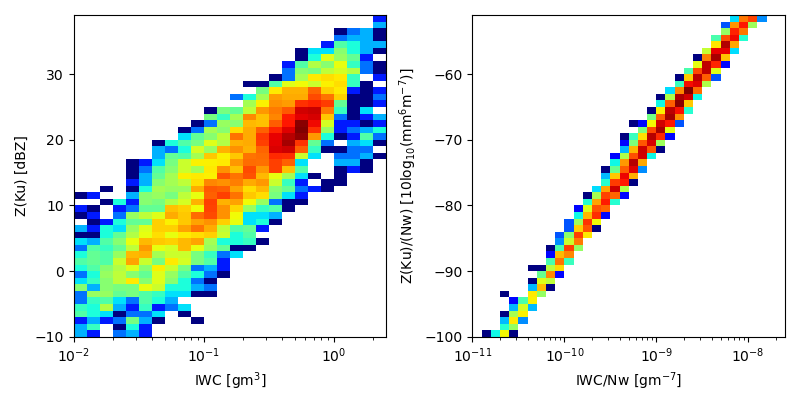
\includegraphics[width=\textwidth]{normZvsnormIWC.png}

\caption{ (Left) joint distribution of ice water content (IWC) and associated Ku-band reflectivity calculated from PSD observations from IMPACTS and
(Right) joint distribution of normalized IWC and Ku-band reflectivity. }
\end{figure}


%\begin{table}[!tb]
%\caption{A table}
%\processtable{ Example of code }
%\lstset{language=Python}
%\lstset{frame=lines}
%\lstset{caption={Insert code directly in your document}}
%\lstset{label={lst:code_direct}}
%\lstset{basicstyle=\footnotesize}
%\begin{lstlisting}
%from brg.datastructures import Mesh
 
%mesh = Mesh.from_obj('faces.obj')
%mesh.draw()
%\end{lstlisting}
%\end{table}

%\subsection{B heading (level 2)}

%\subsubsection{C heading (level 3)}

%\begin{figure}[!b]
%\centerline{\fbox{\hbox to 20pc{\vbox to 10pc{}}}}
%\caption{little figure here}
%\end{figure}

%\paragraph{D heading (level 4)}



\bibliographystyle{vancouver-modified}
\bibliography{sample-vancouver}

\end{document}
